\documentclass[11pt]{article}
\usepackage[left=0.8in, right=0.8in, top=0.6in, bottom=0.6in]{geometry}
\usepackage[T1]{fontenc}
\usepackage[utf8]{inputenc}
\usepackage{lmodern}
\usepackage{setspace}
\usepackage{hyperref}
\usepackage{enumitem}
\usepackage{titlesec}
\usepackage{graphicx}
\usepackage{float}
\usepackage{subcaption}
\usepackage{indentfirst}

\title{\textbf{UM ParkSight: Vision-Based Parking Occupancy Estimation for U-M Lots Using Reference-Image Registration}}
\author{Felix Sixiang Tang \and Keheng Zhu \and Kwan Ting Lau}
\date{}

\begin{document}
\maketitle
\onehalfspacing

\section{Executive Overview}

\textbf{Pipeline Architecture.} UM ParkSight is a lightweight computer vision pipeline that estimates real-time parking occupancy from a single oblique-angle photograph. Rather than relying on embedded sensors or purpose-built overhead cameras, our system registers a one-time manually annotated reference image to new photos via learned feature matching. 

\textbf{Classification and Output.} Each transferred spot region is classified using a pretrained vehicle recognition model. The per-spot results are then rendered onto a top-down occupancy map, offering a highly deployable solution that requires no new infrastructure beyond a single elevated vantage point.

\begin{figure}[H]
    \centering
    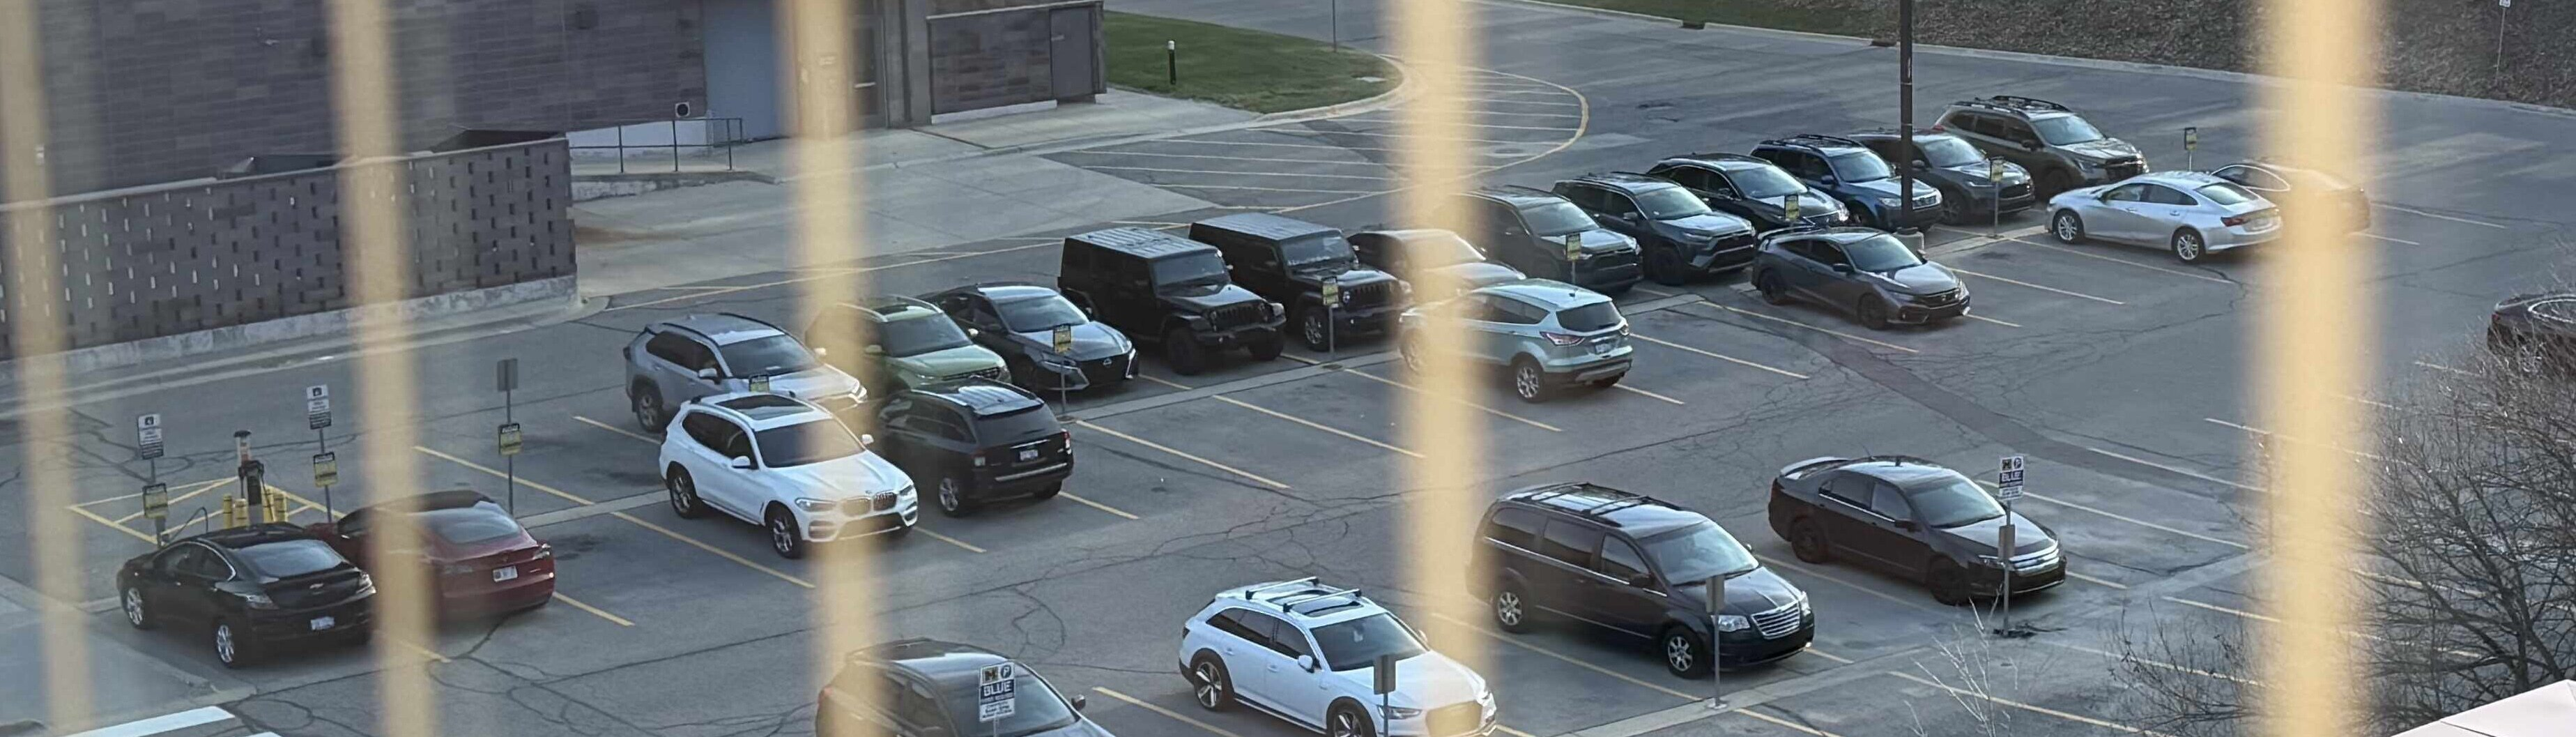
\includegraphics[width=0.48\textwidth]{figures/reference_image.jpg}
    \hfill
    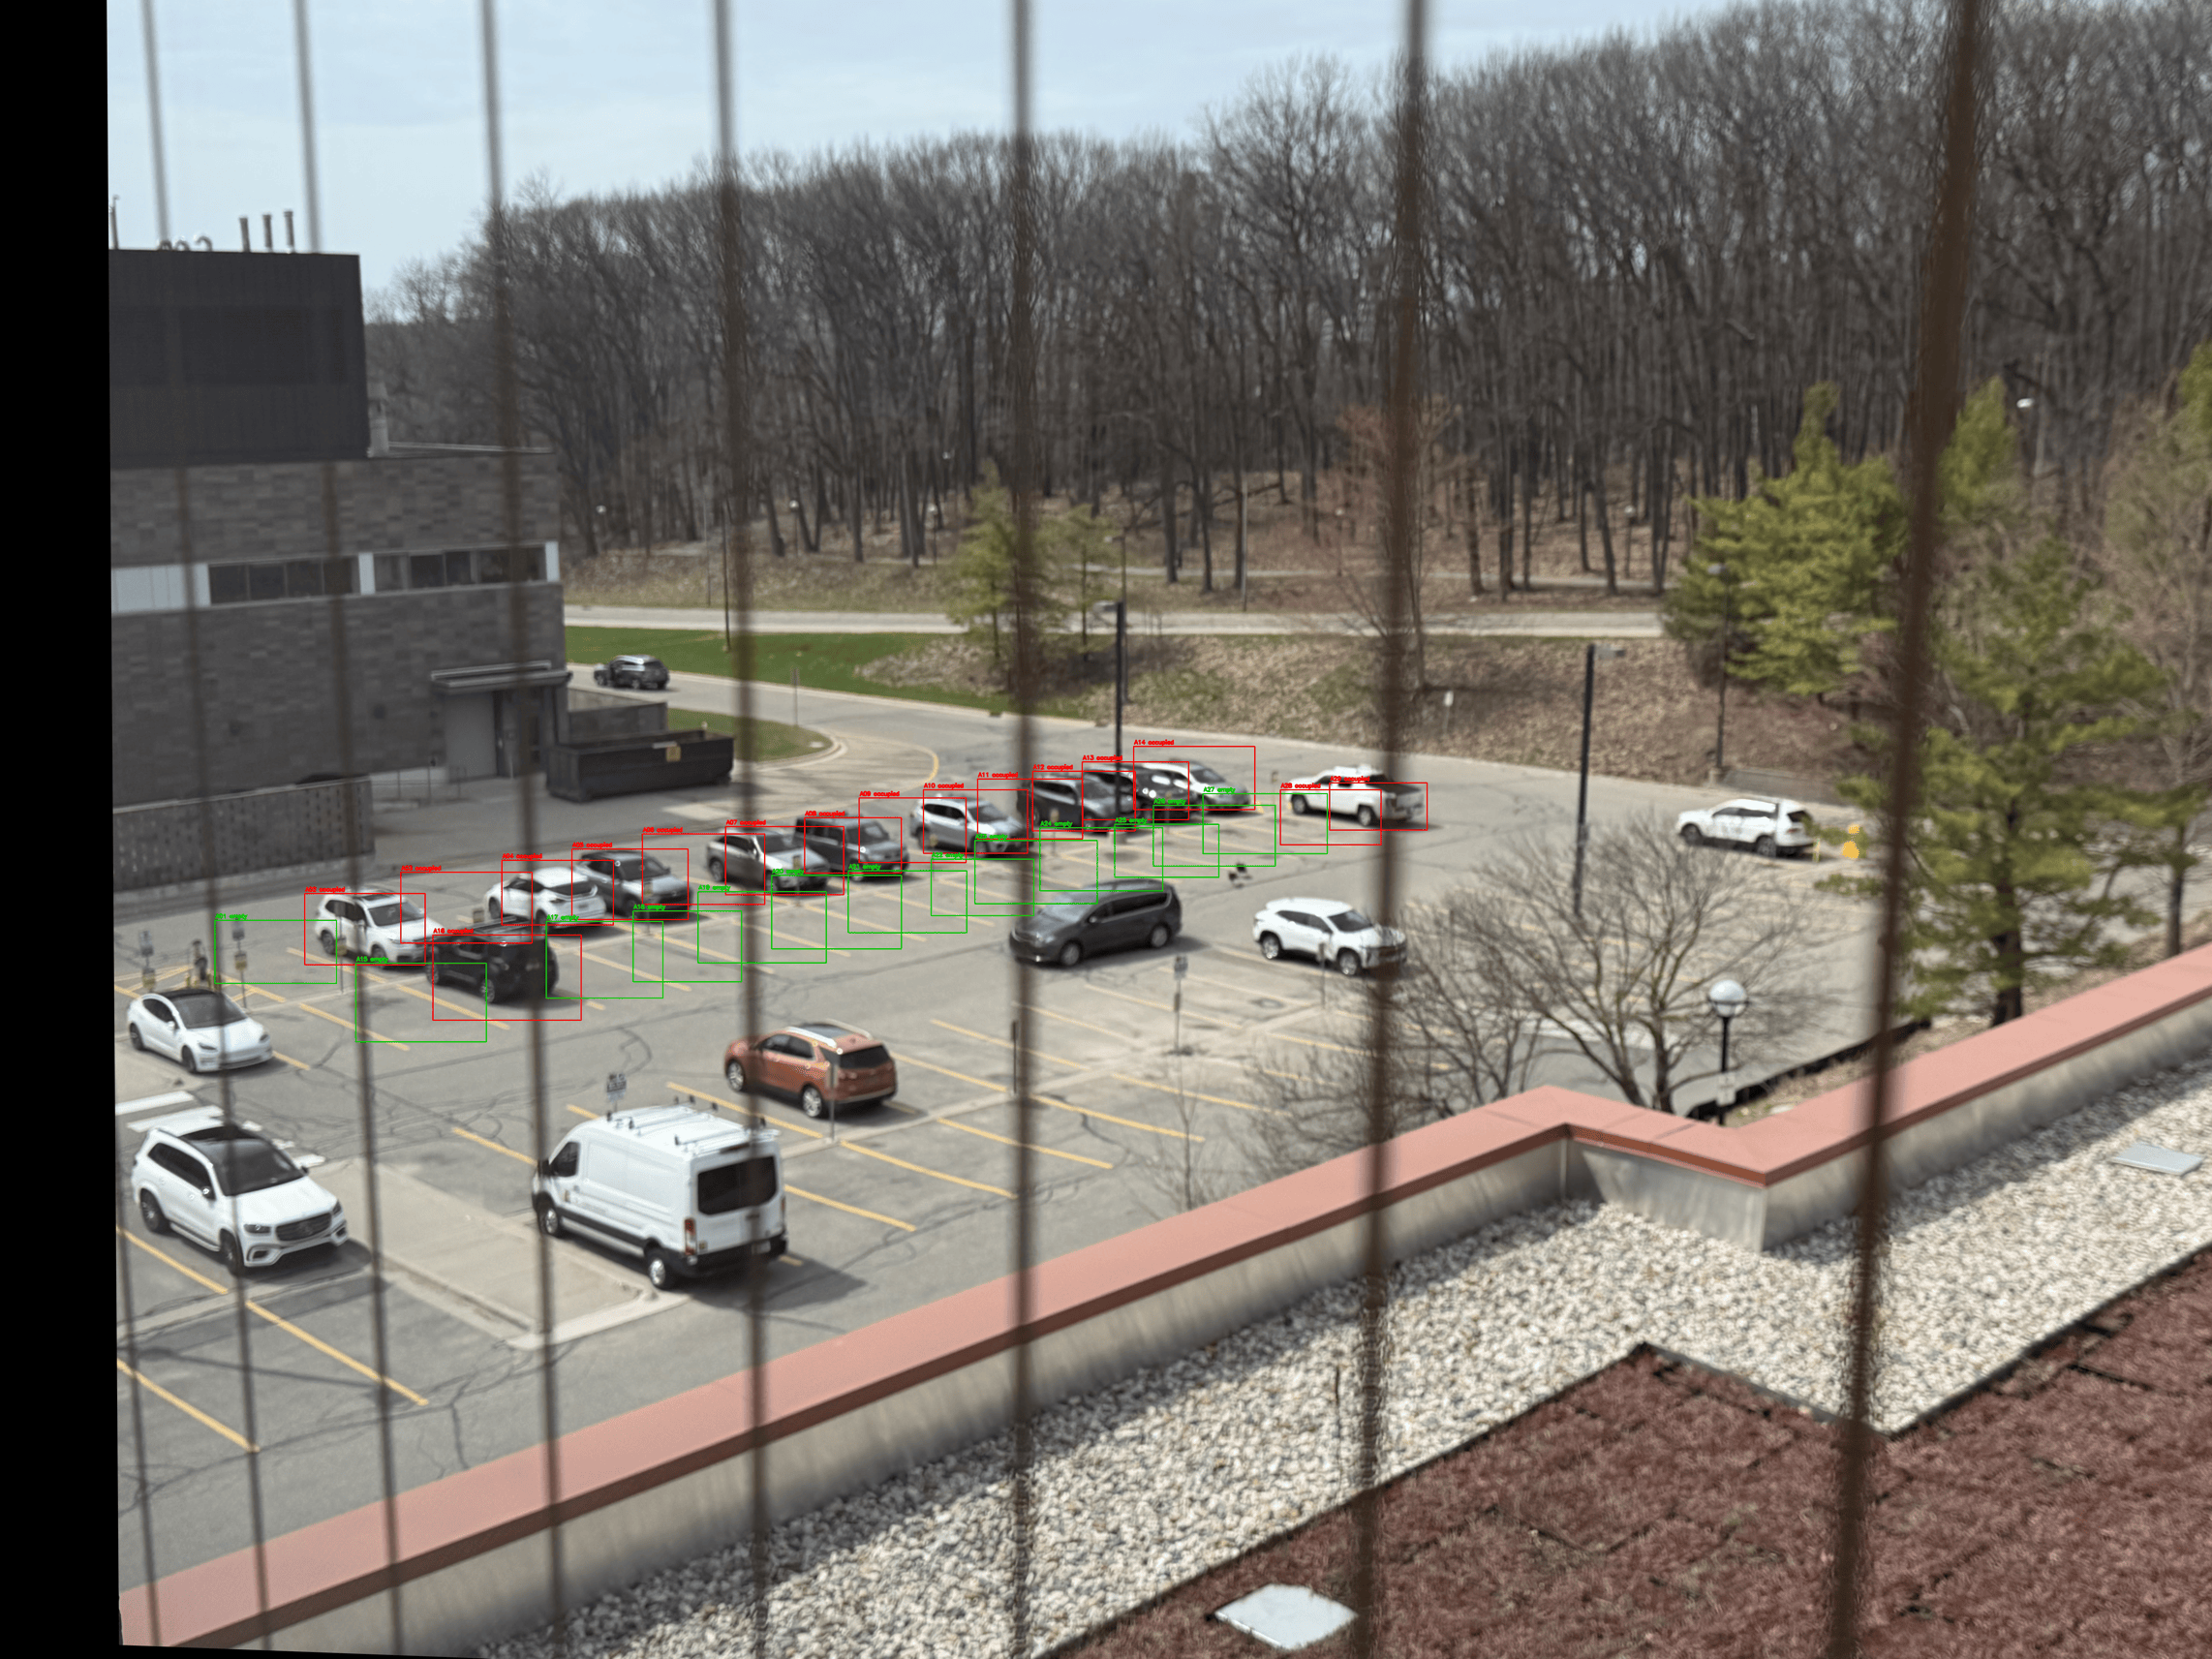
\includegraphics[width=0.48\textwidth]{figures/resolved_occupancy_overlay.png}
    \caption{System overview example. Left: reference lot image used for one-time spot annotation. Right: final occupancy overlay produced by the pipeline (green: empty, red: occupied).}
    \label{fig:overview_input_output}
\end{figure}

\section{Background and Impact}
\textbf{The Cruising Problem.} In 2017, a study involving nearly 18,000 drivers found that US drivers spend an average of 17 hours per year searching for parking, meaning \$345 annually per driver, totaling around \$73 billion nationally \cite{parkingstudy2017}. At the University of Michigan, this translates to familiar frustrations for students and staff circling peak-hour lots, uncertain if any spaces remain.

\textbf{Limitations of Existing Solutions.} Current systems fall into two inadequate extremes. Gate-based counters only track aggregate occupancy, failing to tell drivers \emph{where} open spots are (leading to internal lot cruising). Conversely, per-space sensor arrays (magnetometers, ultrasonics) provide granular data but demand expensive hardware and high maintenance that smaller or older lots cannot justify.

\textbf{Our Contribution and Impact.} UM ParkSight targets this gap. By utilizing a single existing building camera and one-time calibration, we provide per-space data comparable to sensor arrays at a fraction of the cost. Our twofold intended impact is reducing driver cruising time (and associated emissions) and offering a low-barrier path for under-instrumented facilities—like many U-M surface lots—to provide real-time availability data.

\section{Method}
Our pipeline consists of four stages:
\begin{enumerate}[leftmargin=1.5em]
    \item \textbf{Reference Annotation.} A one-time setup where the visible parking spots in a single elevated oblique reference image are manually outlined as quadrilateral regions and saved as a JSON template.
    
    \item \textbf{Registration via LoFTR.} To handle variations in viewpoint or time of day, we use LoFTR, a detector-free local feature transformer \cite{sun2021loftr}, to establish dense correspondences between the reference and new query images. LoFTR excels in low-texture regions (e.g., asphalt) where classical detectors like SIFT often fail. We use these matches to estimate a homography and warp the annotated spot polygons into the query frame.
    
    \item \textbf{Per-Spot Occupancy Classification.} Direct vehicle detection fails frequently on steep, dense oblique views. Instead, we crop each warped polygon and pass it to a pretrained fine-grained car classifier (Stanford\_Car \cite{roboflow_stanford_car}). By reframing the model as a simple car-presence detector on framed imagery, we bypass the need to collect massive amounts of lot-specific training data. Confident predictions are marked occupied.
    
    \item \textbf{Top-Down Occupancy Map.} Spot classifications are projected onto a 2D schematic map (green for available, red for occupied) to create a glanceable end-user interface.
\end{enumerate}

\begin{figure}[htbp]
    \centering
    % Row 1: LoFTR Registration
    \begin{subfigure}{0.64\textwidth}
        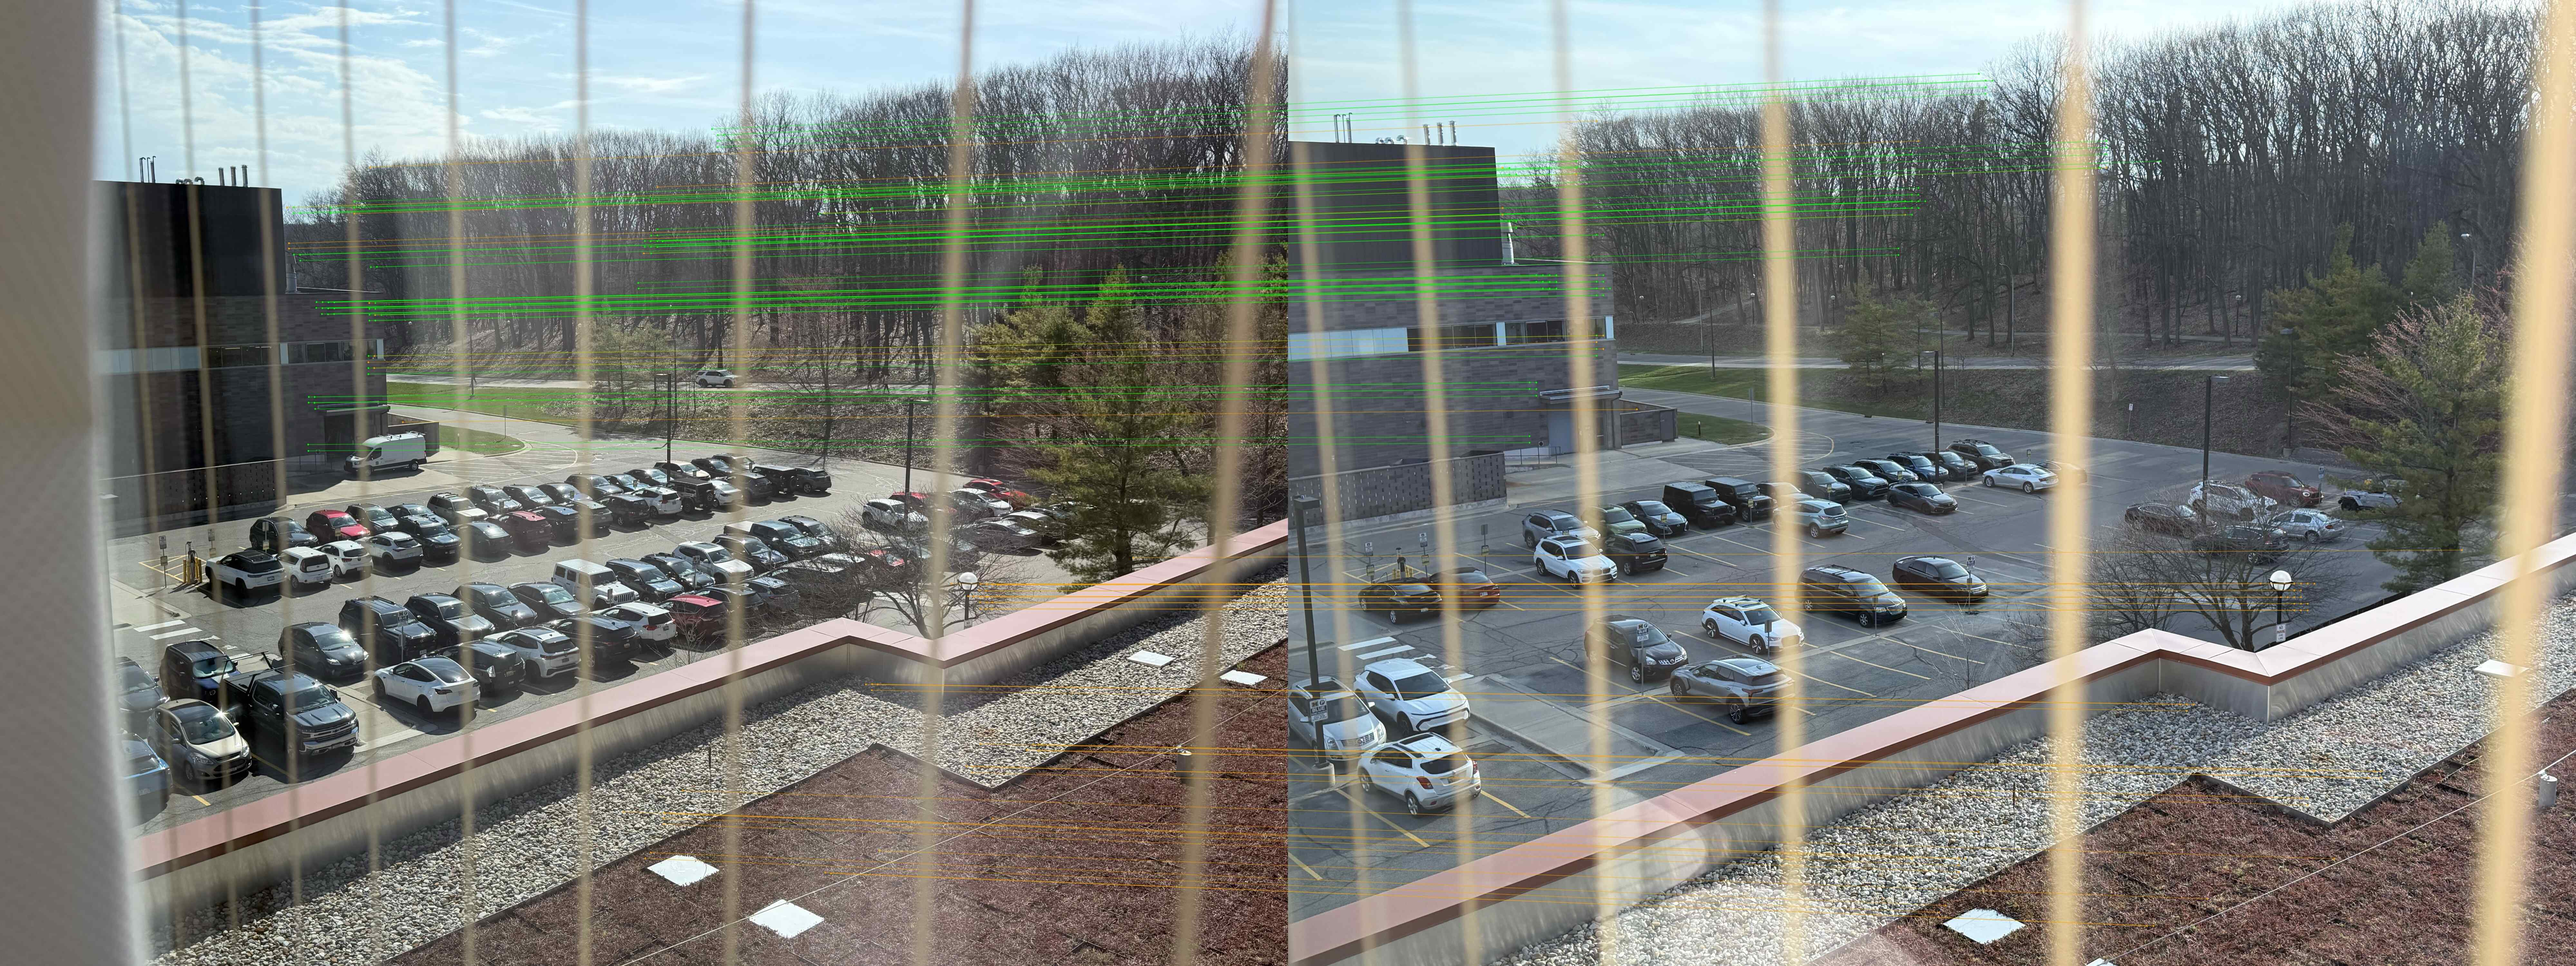
\includegraphics[width=\textwidth]{figures/loftr_matches_query.jpg}
        \caption{LoFTR feature correspondences}
    \end{subfigure}
    \hfill
    \begin{subfigure}{0.32\textwidth}
        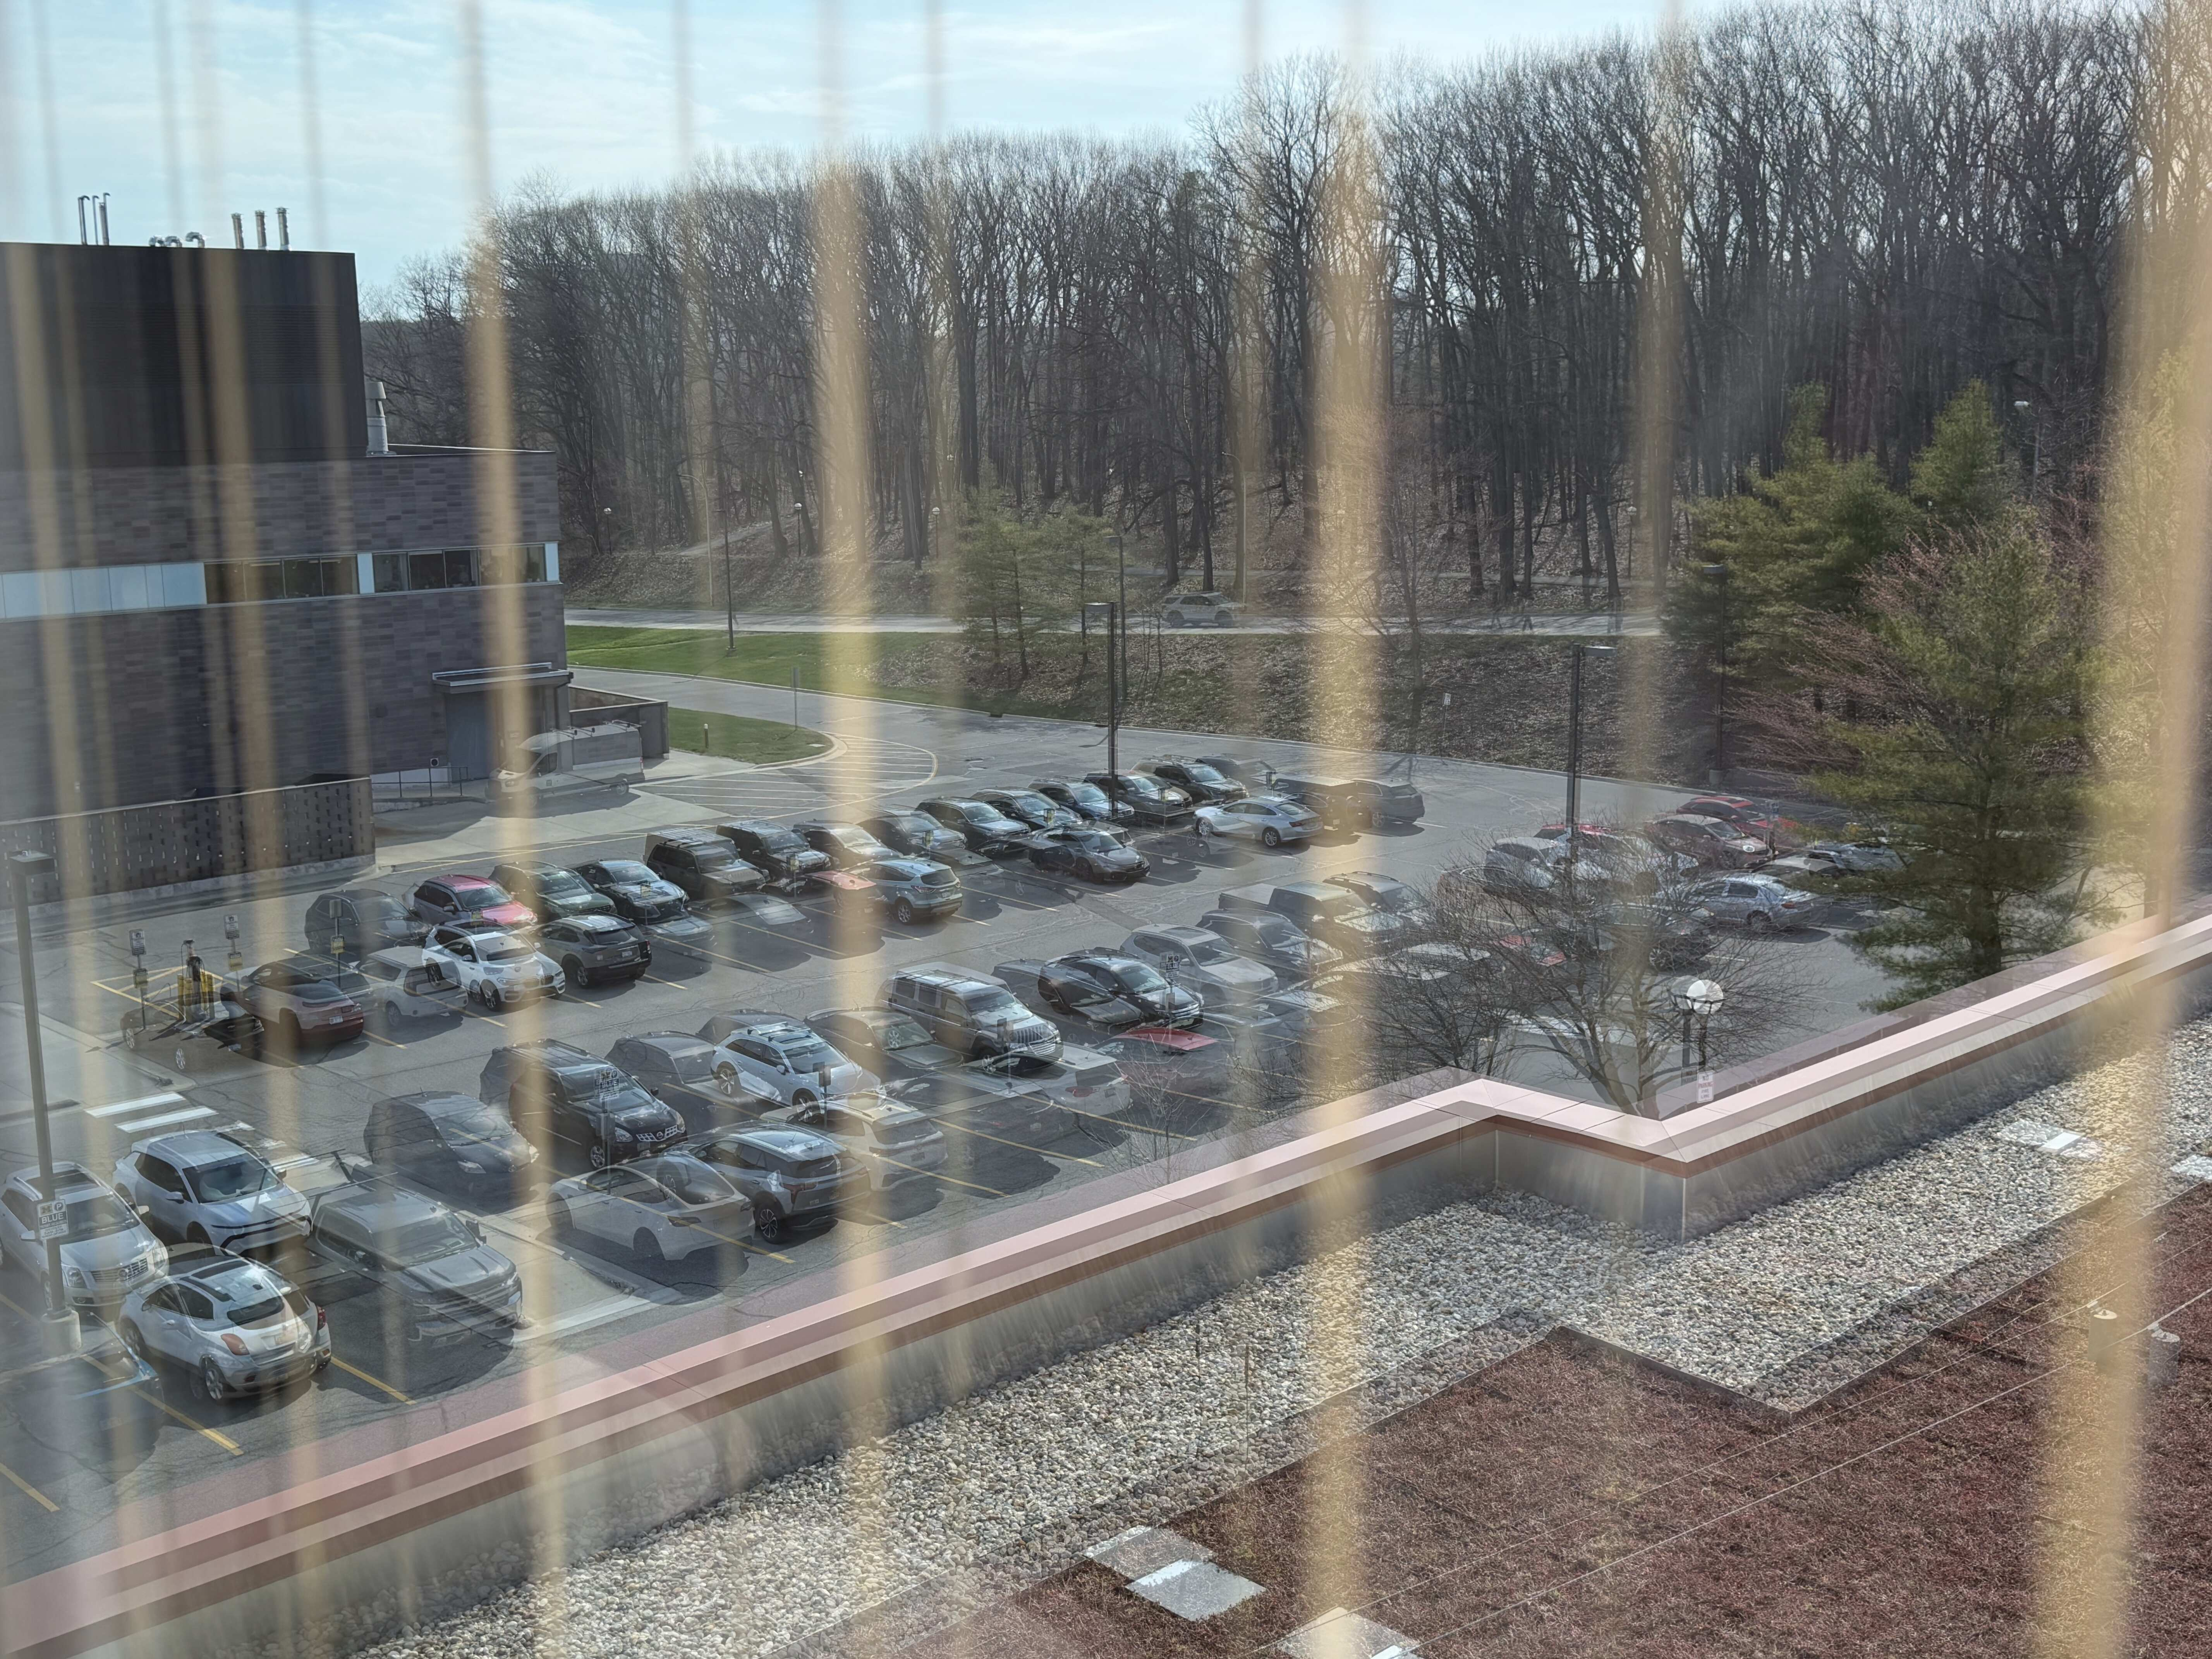
\includegraphics[width=\textwidth]{figures/registration_overlay.jpg}
        \caption{Alignment overlay}
    \end{subfigure}
    
    \vspace{0.4cm}
    
    % Row 2: Crops and Map
    \begin{subfigure}{0.58\textwidth}
        \centering
        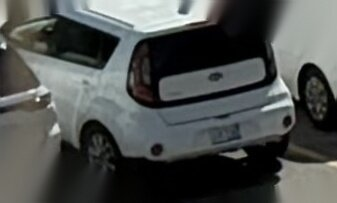
\includegraphics[width=0.31\textwidth]{figures/spot_occupied_example.jpg}
        \hfill
        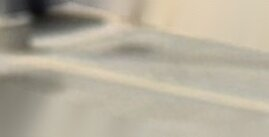
\includegraphics[width=0.31\textwidth]{figures/spot_empty_example.jpg}
        \hfill
        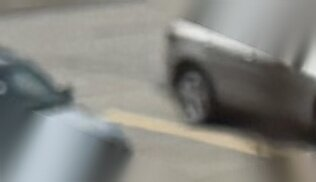
\includegraphics[width=0.31\textwidth]{figures/spot_borderline_example.jpg}
        \caption{Per-spot crops (occupied, empty, borderline)}
    \end{subfigure}
    \hfill
    \begin{subfigure}{0.4\textwidth}
        \centering
        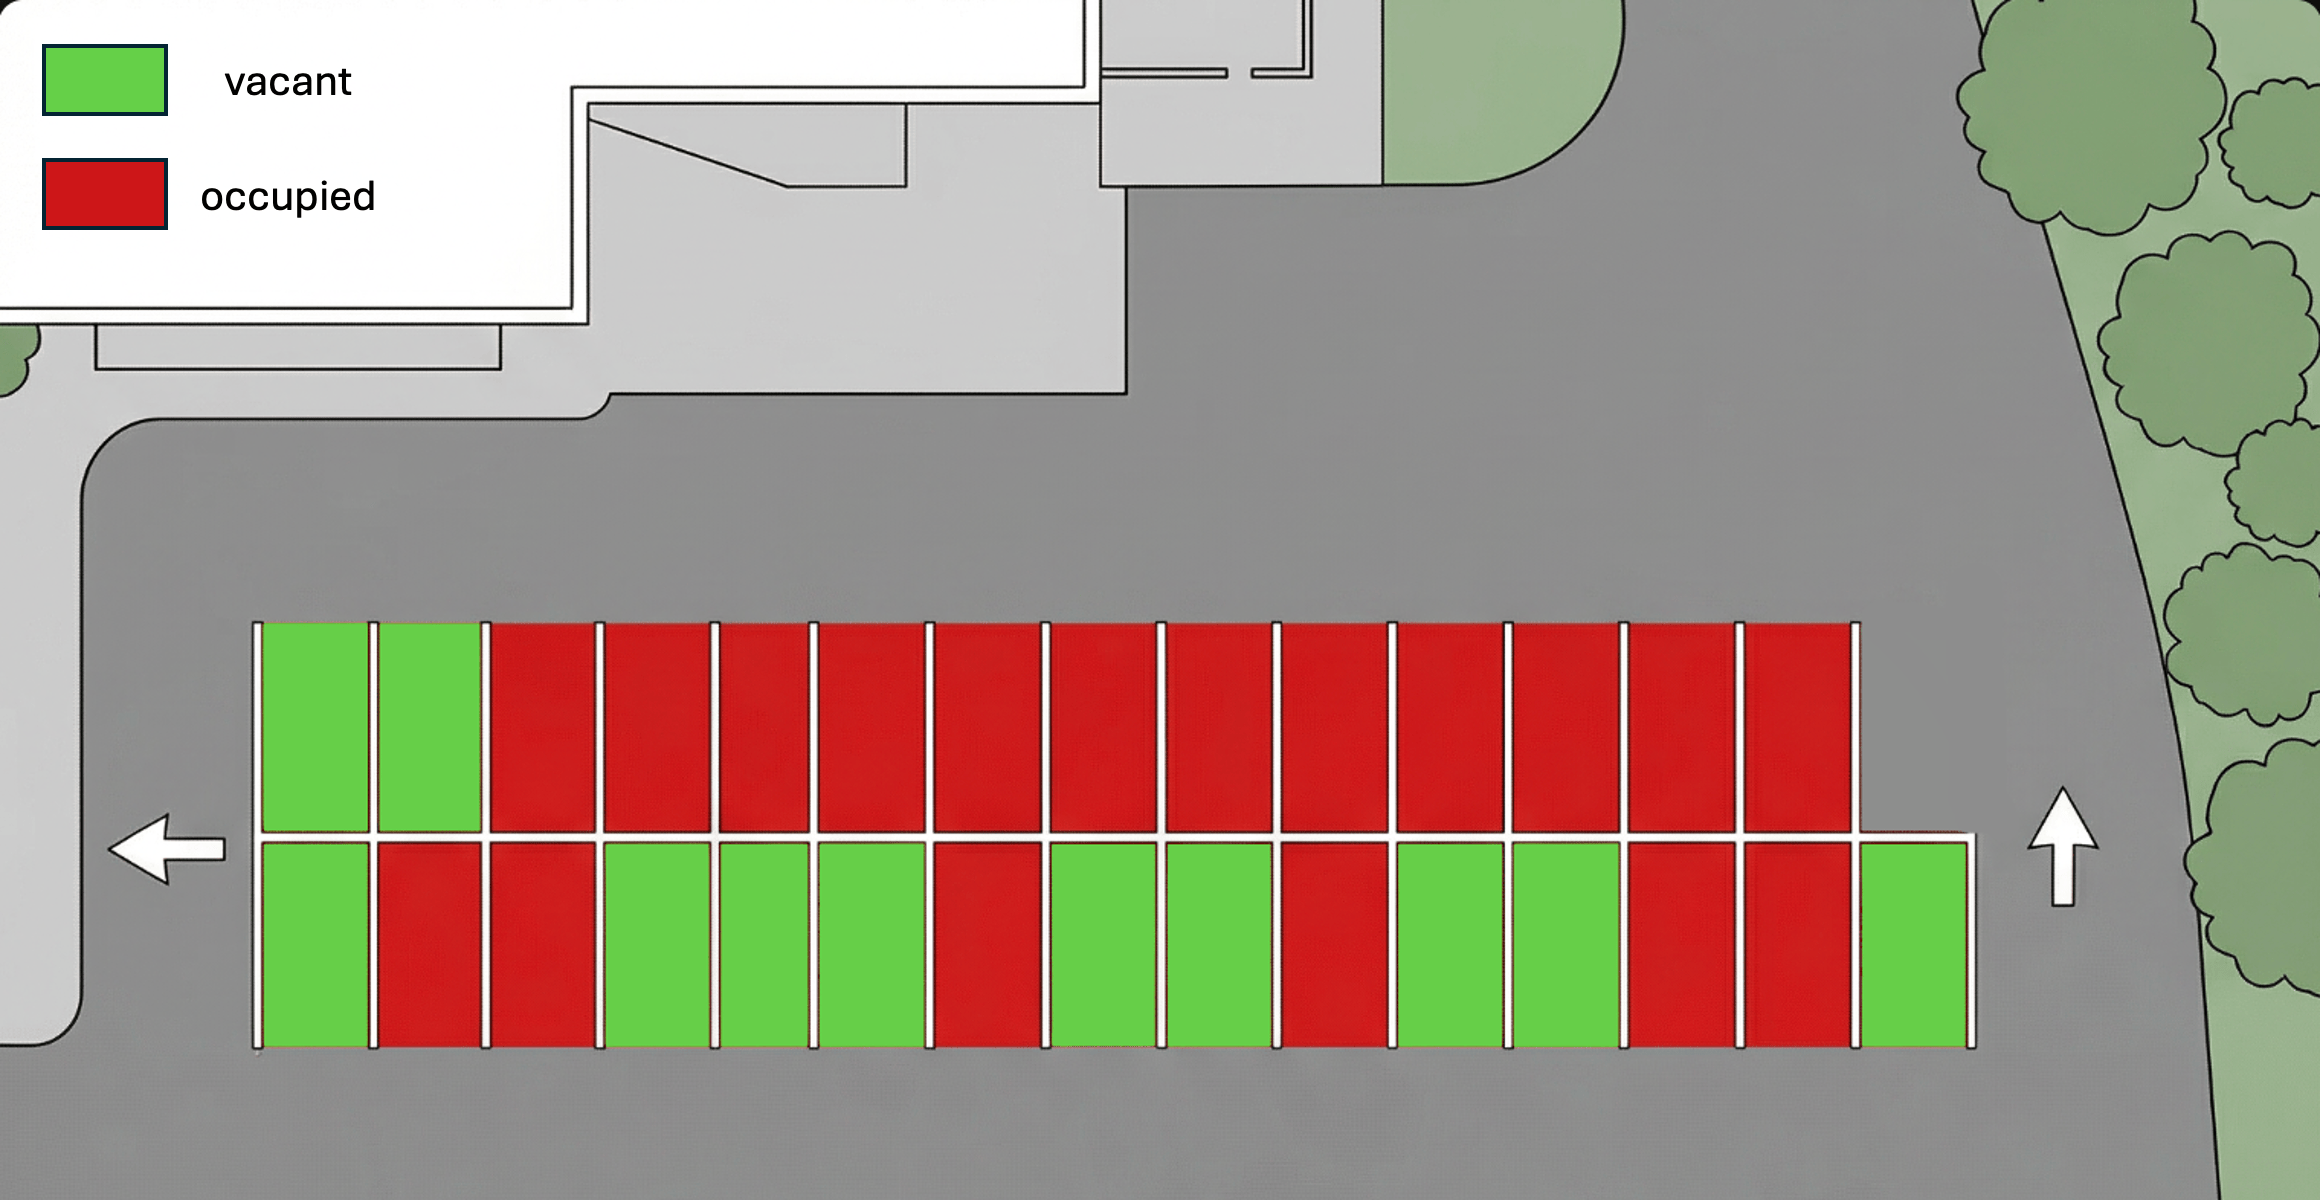
\includegraphics[width=0.8\textwidth]{figures/2D_map.png}
        \caption{Final 2D glanceable map}
    \end{subfigure}
    
    \caption{Methodology pipeline: (a-b) Reference-to-query registration via homography warping, (c) cropped inputs for the occupancy classifier, and (d) the final top-down artifact.}
    \label{fig:methodology_pipeline}
\end{figure}

\section{Prototype}

\textbf{Initial Approaches and Limitations.} Our initial approach attempted direct car detection on oblique lot photos using several pretrained object detectors. However, performance was poor due to a domain mismatch: standard models generalize poorly to the steep, densely packed, and partially occluded oblique views in our scenario. We then explored automatically extracting parking spot boundaries from painted lines, but the lines in our reference imagery were frequently occluded by vehicles, shadowed, or faded, making robust line detection unreliable.

\begin{figure}[H]
    \centering
    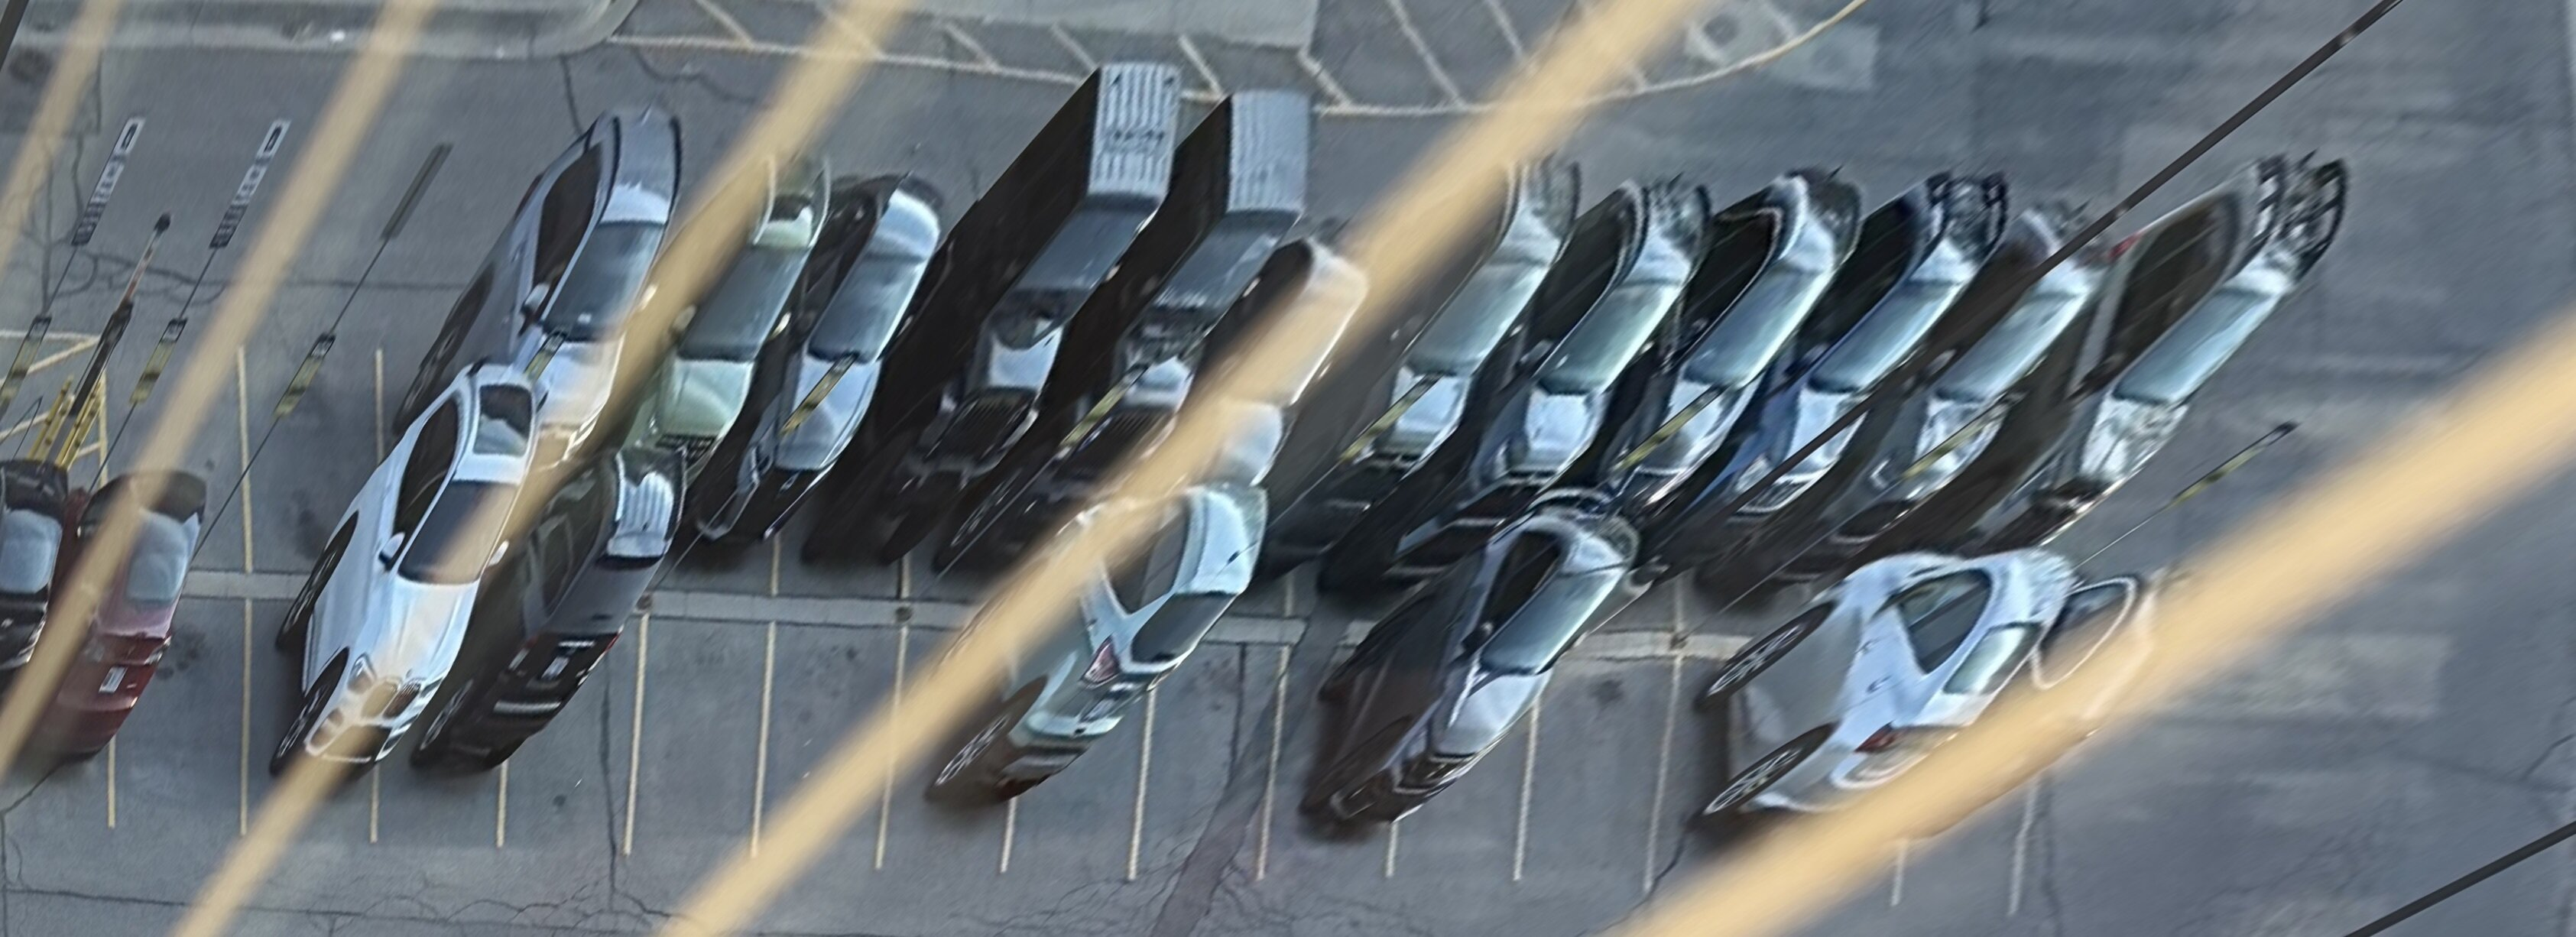
\includegraphics[width=0.6\textwidth]{figures/prototype_direct_detection_failure.jpg}
    \caption{Prototype-stage failure mode: Direct vehicle detection on oblique scenes produced unstable results.}
    \label{fig:prototype_failures}
\end{figure}

\textbf{Revised Design: Per-Spot Classification.} These challenges led to our current design: while detecting cars \emph{in context} is difficult, classifying \emph{whether a tight crop contains a car} is highly reliable. This shifted the problem from ``find the cars'' to ``find the spots, then ask about each spot''. This approach reduces the complex detection task to an image registration problem, where manual spot annotation serves as a reasonable, one-time calibration step per lot.

\textbf{Implementation Details.} The final prototype is implemented in Python, utilizing LoFTR weights for feature matching, OpenCV for homography estimation and warping, and the Roboflow inference API for classification. All code for this project is publicly available in our open-source GitHub repository at \url{https://github.com/KehengZhu/UM-ParkSight}.

\section{Results}
We ran the complete notebook pipeline (alignment, interactive spot translation, per-spot cropping, detector inference, and rule-based occupancy resolution) on representative query images from the same lot. Figure \ref{fig:segment_detection_grid} shows the crop-level detector outputs used as inputs to final occupancy decisions.

\begin{figure}[H]
    \centering
    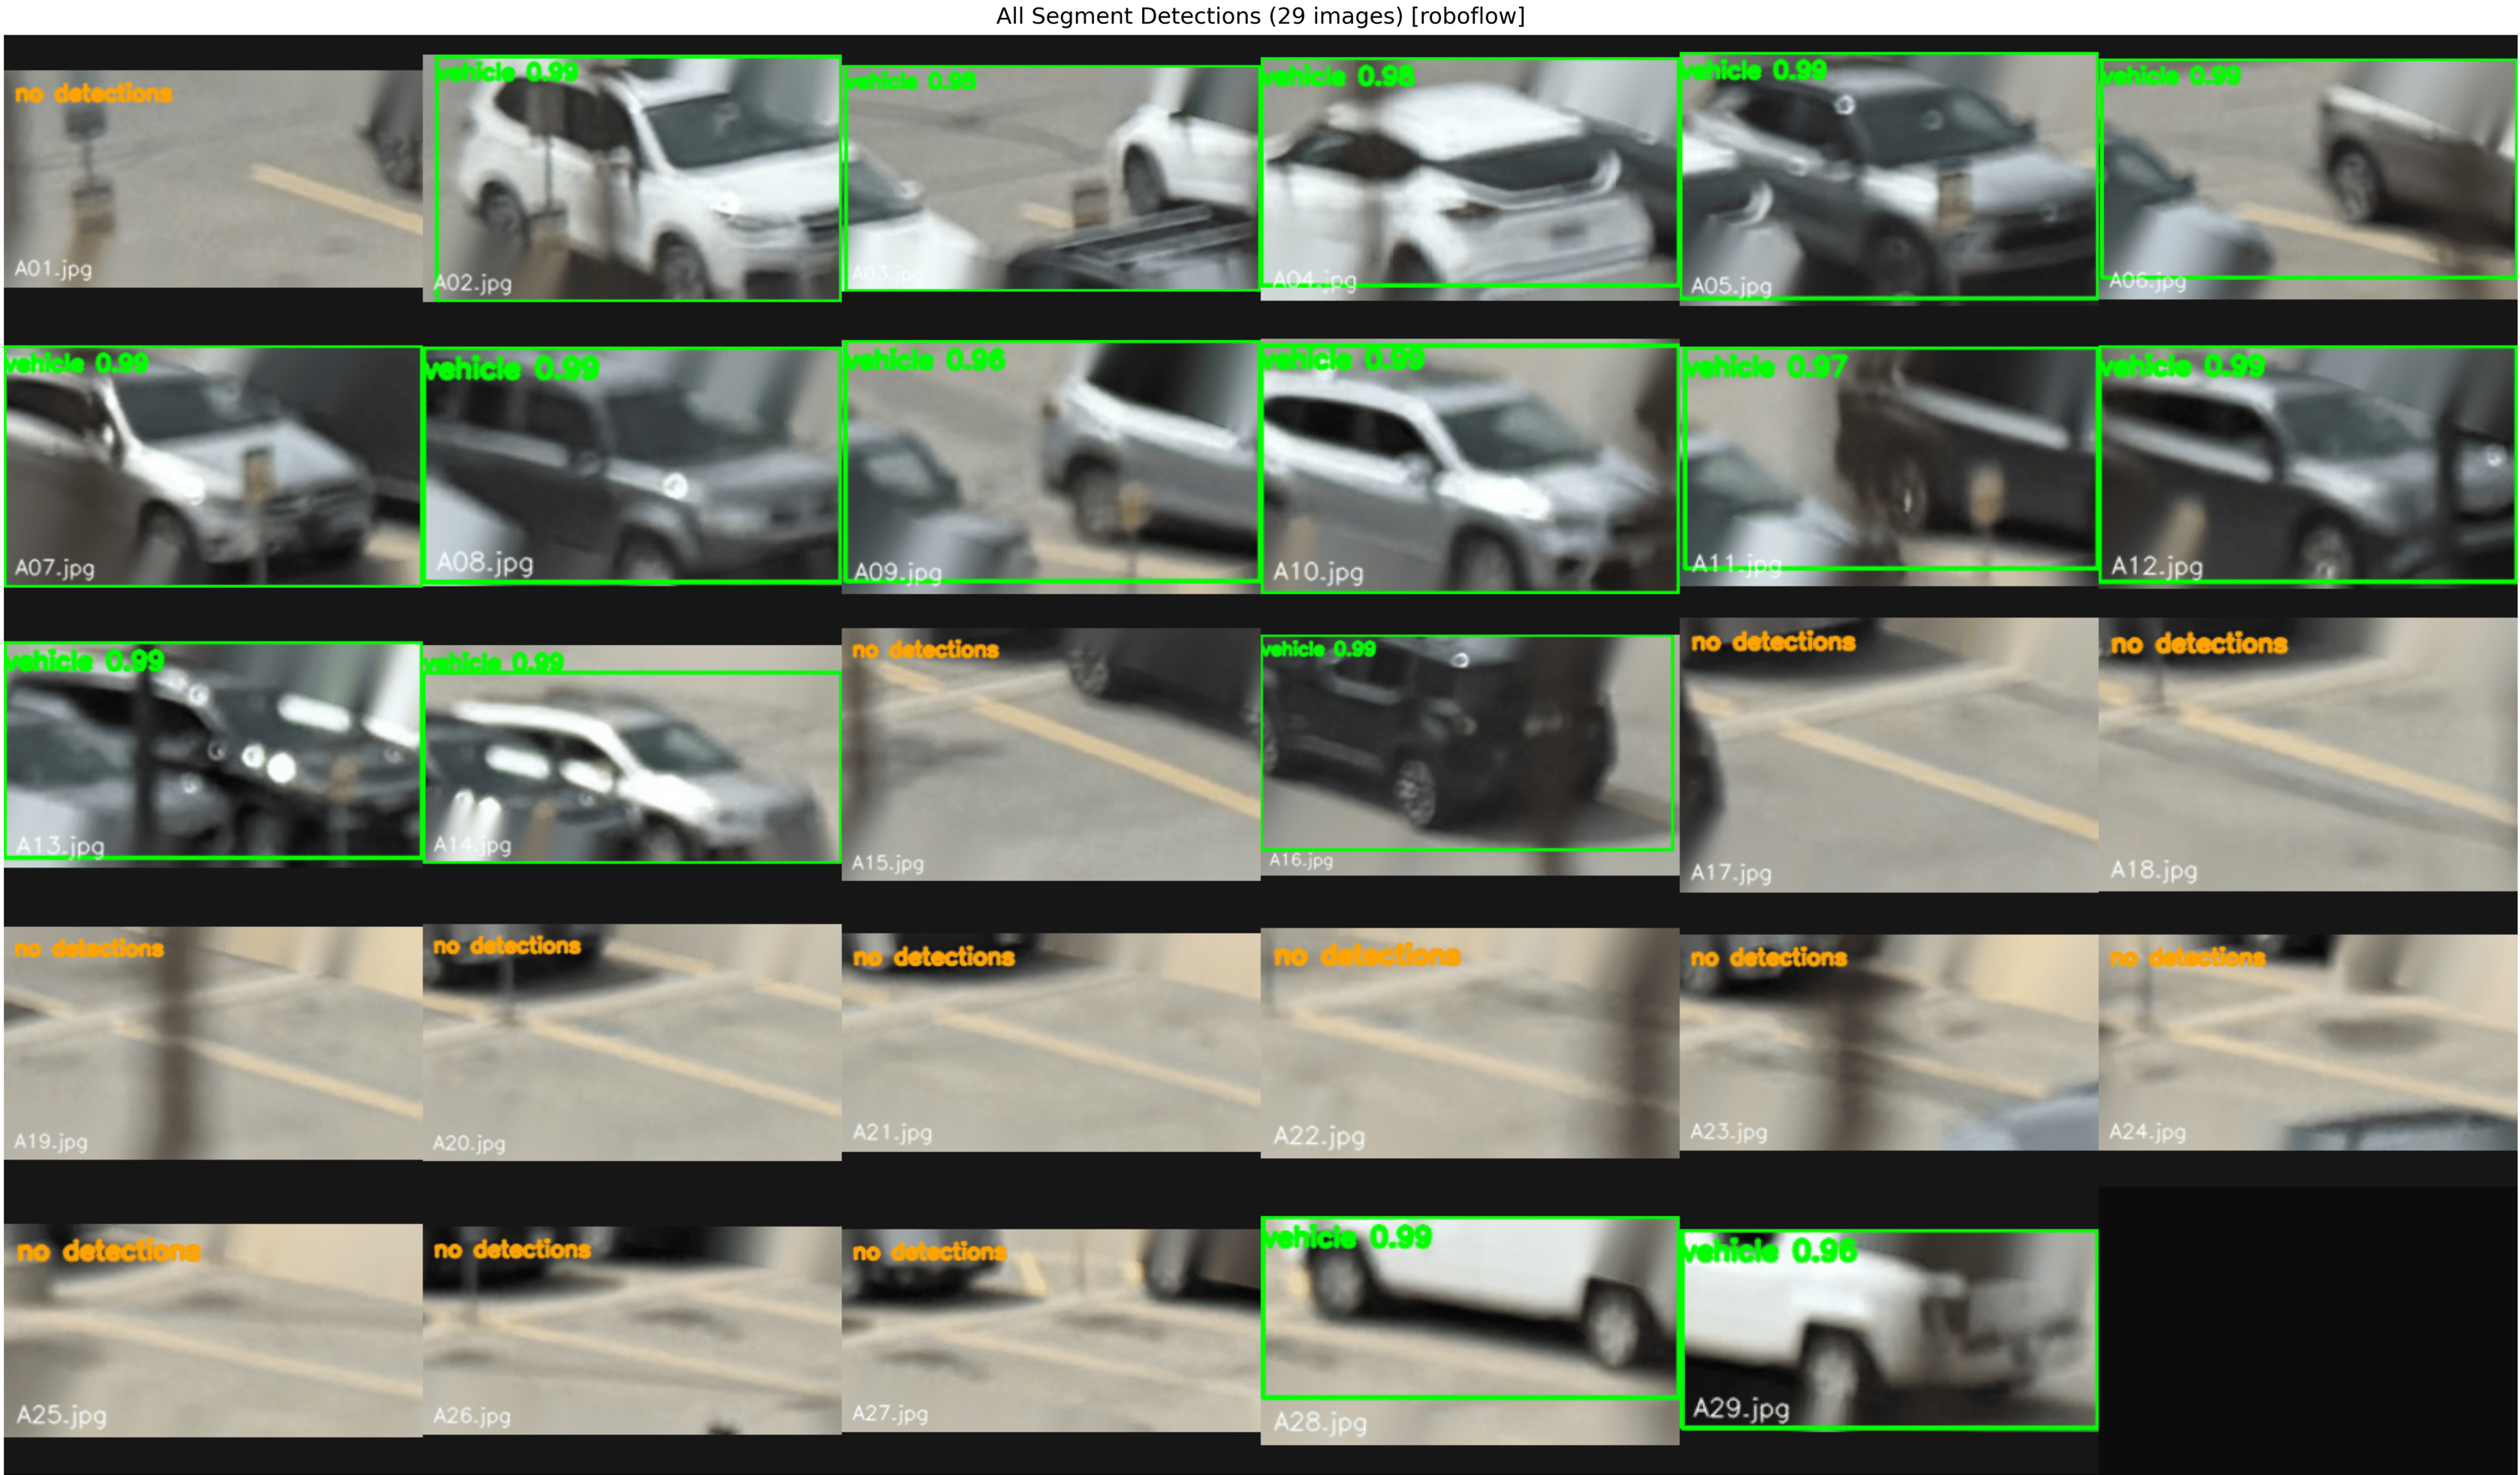
\includegraphics[width=0.6\textwidth]{figures/segment_detection_grid.png}
    \caption{Per-spot detection grid generated by the notebook pipeline. Each tile corresponds to one parking spot crop with detector predictions overlaid.}
    \label{fig:segment_detection_grid}
\end{figure}

For the resolved output corresponding to reference image stored in resolved\_occupancy.json, the system processed 29 parking spots, labeling 16 as occupied and 13 as empty, corresponding to a measured occupancy rate of 55.17\%. The mean confidence among occupied spots was 0.985, and all occupied spots in this run passed the strict center-and-area gate. Among strict-pass occupied spots, the mean bounding-box area ratio was 0.937.

To supplement these operational metrics, we also evaluated the pipeline against manually annotated test images representing different lot states, summarizing our performance findings in Figure \ref{fig:performance_results}.

\begin{figure}[H]
    \centering
    \begin{subfigure}[t]{0.31\textwidth}
        \centering
        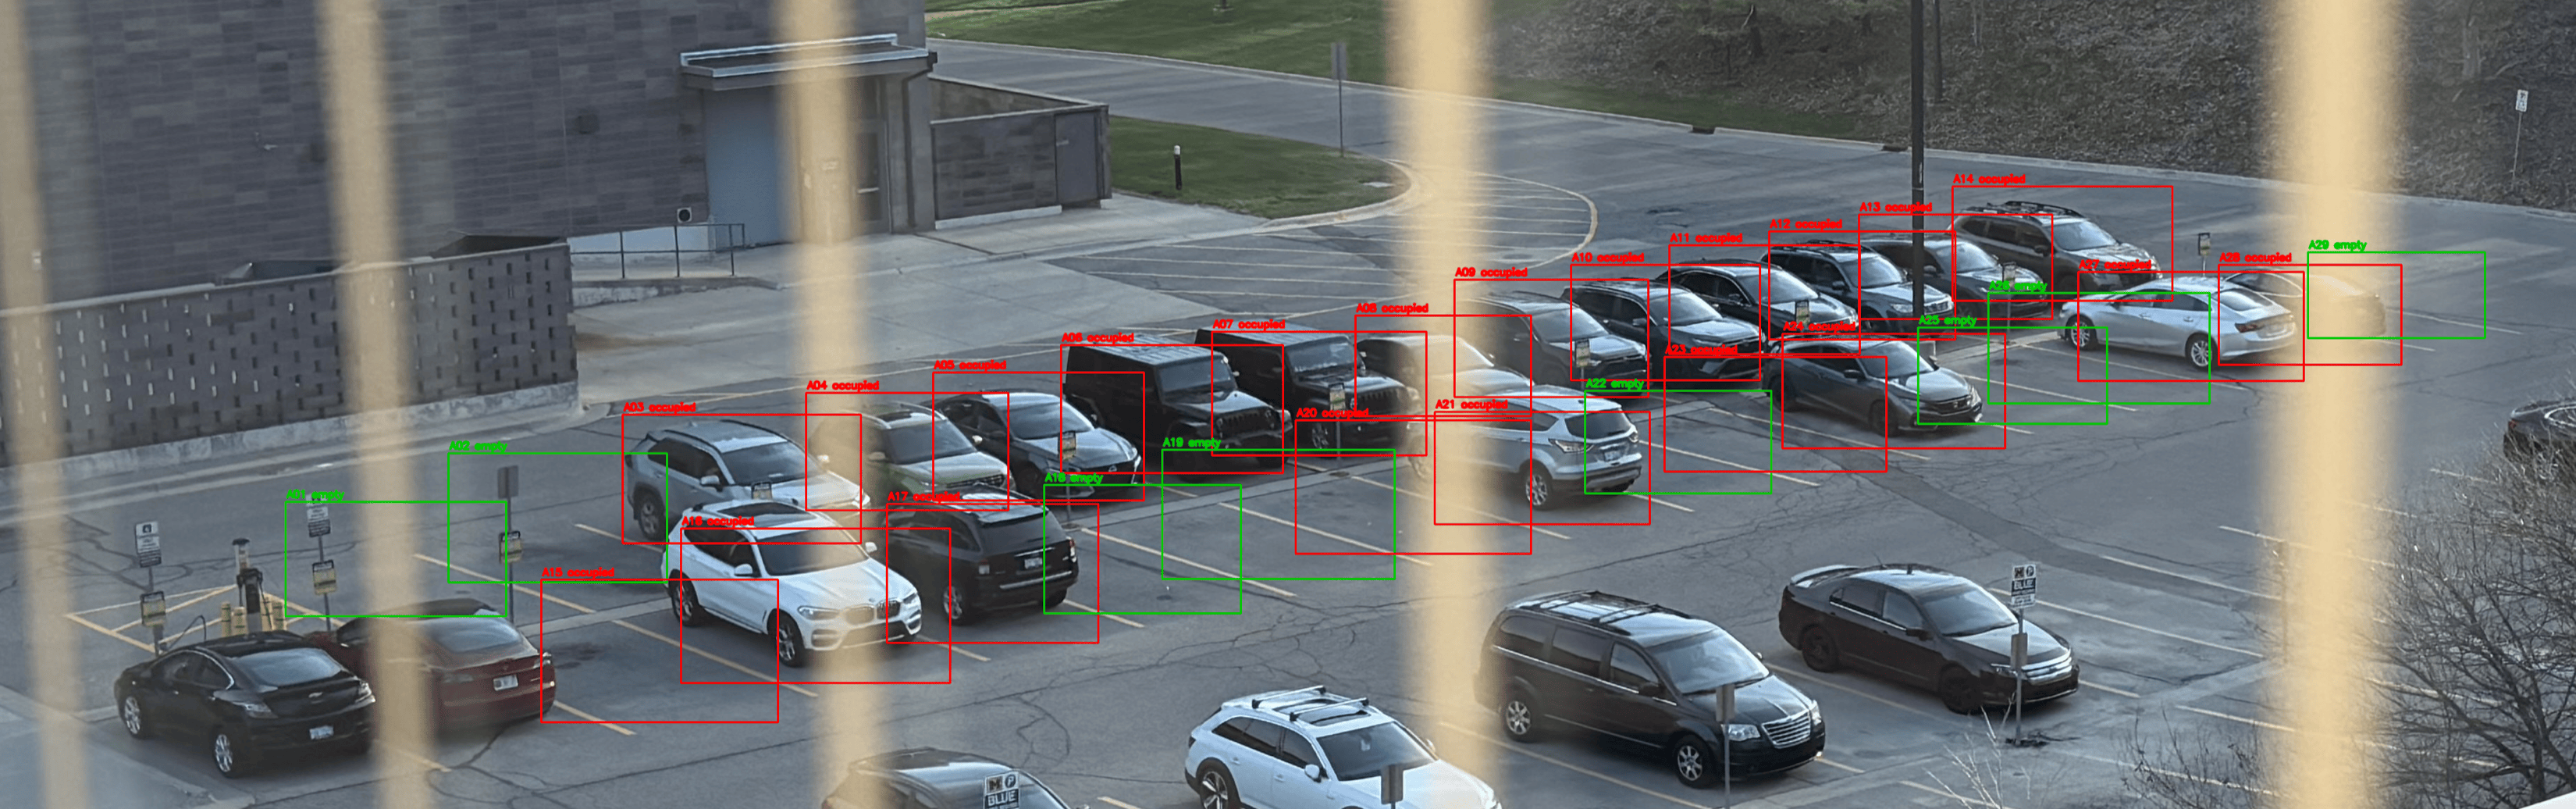
\includegraphics[width=\textwidth]{figures/results_reference.png}
        \caption*{Reference Image}
        \vspace{0.2cm}
        \begin{tabular}{@{}l l@{}}
            Total spots: & 29 \\
            Accuracy: & 89.7\% \\
            False pos: & 3/29 \\
            False neg: & 0/29 \\
        \end{tabular}
    \end{subfigure}
    \hfill
    \begin{subfigure}[t]{0.31\textwidth}
        \centering
        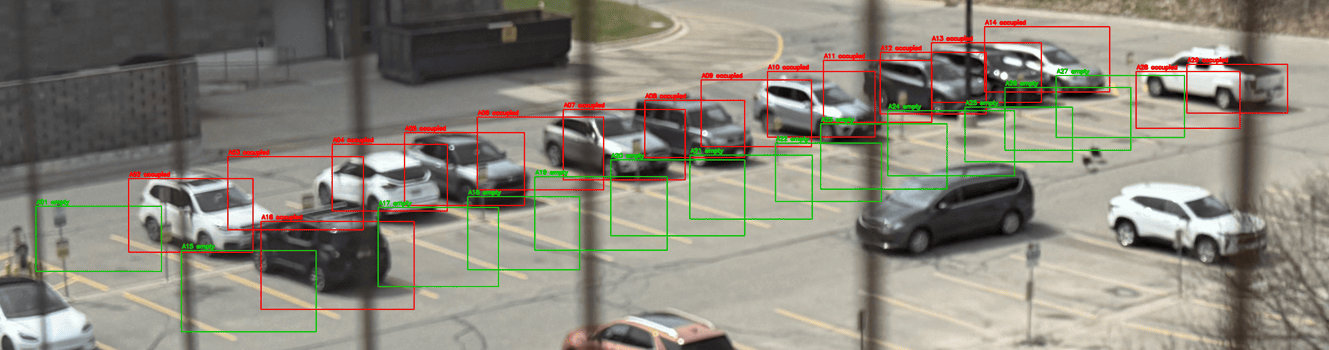
\includegraphics[width=\textwidth]{figures/results_empty_lot.png}
        \caption*{Test Image 1: Empty lot}
        \vspace{0.2cm}
        \begin{tabular}{@{}l l@{}}
            Total spots: & 29 \\
            Accuracy: & 82.7\% \\
            False pos: & 5/29 \\
            False neg: & 0/29 \\
        \end{tabular}
    \end{subfigure}
    \hfill
    \begin{subfigure}[t]{0.31\textwidth}
        \centering
        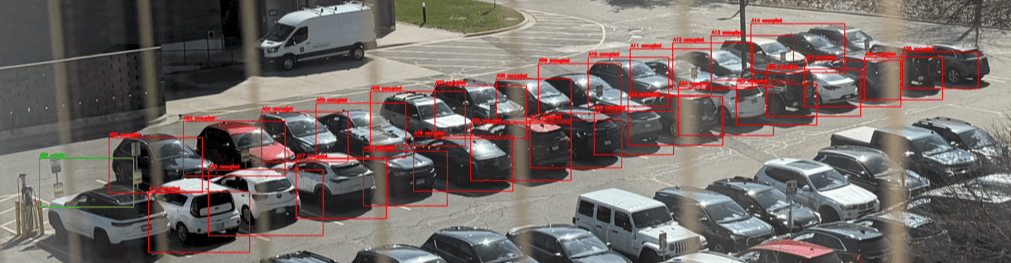
\includegraphics[width=\textwidth]{figures/results_full_lot.png}
        \caption*{Test Image 2: Full lot}
        \vspace{0.2cm}
        \begin{tabular}{@{}l l@{}}
            Total spots: & 29 \\
            Accuracy: & 100.0\% \\
            False pos: & 0/29 \\
            False neg: & 0/29 \\
        \end{tabular}
    \end{subfigure}
    \caption{Performance evaluation across the reference image and test sets with varying lot occupancies.}
    \label{fig:performance_results}
\end{figure}

\section{Conclusion}
UM ParkSight demonstrates that per-space parking occupancy estimation can be achieved using only a single elevated camera view, one-time manual annotation, and learned image registration. By replacing specialized parking hardware with a lightweight vision pipeline, the system offers a practical path toward scalable, low-cost lot monitoring. Future work will focus on larger-scale evaluation, robustness under lighting and weather changes, and improving the occupancy classifier for ambiguous cases, particularly for vacant spots situated tightly between two occupied spots.

\bibliographystyle{plain}
\bibliography{references}
\end{document}